%\begin{frame}
%  \begin{block}{Considerações Finais}
%  \begin{itemize}
%    \item \small Realização de um estudo acerca do agendamento de cargas domésticas
%    \item \small Prospota de um mecanismo de escalonamento usando o CSA
%    \item \small Os resultados indicam que o CSA é mais eficiente para o escalonamento de cargas deslocáveis domésticas quando comparado ao GA
%    \item \small Os resultados indicam que o CSA é mais eficiente para o escalonamento de cargas deslocáveis no sistema proposto, fornecendo uma redução na carga nos horários de pico, diminuindo a relação pico-média (PAR) da demanda
%  \end{itemize}
%    %\begin{itemize}
%      %\item \small Realização de um estudo acerca do agendamento de cargas domésticas
%      %\item \small Proposta de um mecanismo de escalonamento usando o CSA
%      %\item \small Os resultados indicam que o CSA é mais eficiente para o escalonamento de cargas deslocáveis ​​domésticas quando comparado ao GA
%      %\item \small Os resultados obtidos revelam que o escalonamento das cargas deslocáveis ​​via sistema proposto fornece redução de carga de pico e diminui a relação pico-média (PAR) da demanda.
%    %\end{itemize}
%  \end{block}
%\end{frame}

\begin{frame}
  \begin{block}{}
    \begin{itemize}
        \item Melhor realocação das cargas para horários com demanda menor.
        \item Melhor resultado entre os algoritmos com $22\%$ de redução no
          horário de pico de demanda, sendo o CSA melhor em relação ao AG.
    \end{itemize}
  \end{block}
  \begin{figure}[h]
  	\begin{center}
      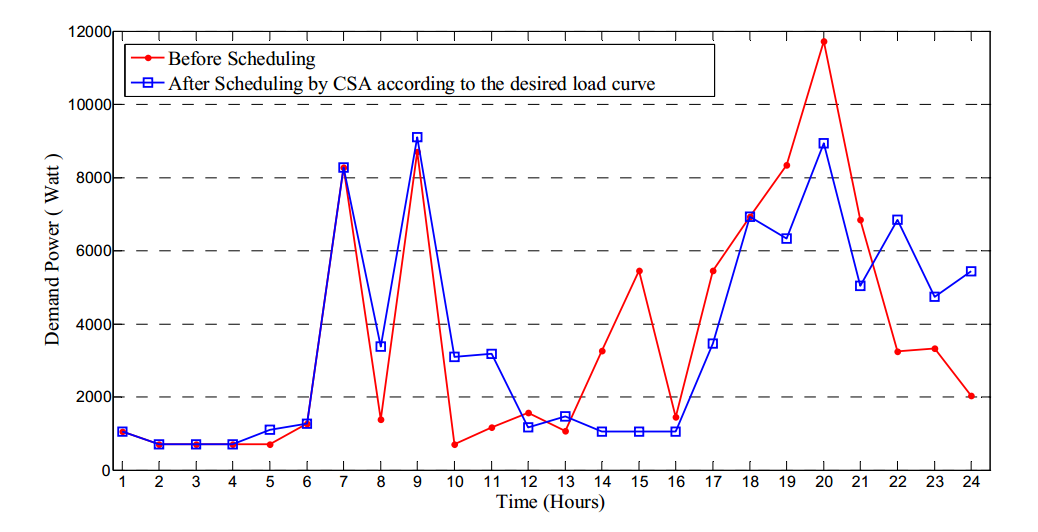
\includegraphics [scale=0.3]{./Figures/t01}
  	\end{center}
  \end{figure}
\end{frame}

\begin{frame}
  \begin{block}{}
   \begin{itemize}
     \item Relatório de estudo de demandas da Empresa de Pesquisa energética EPE.
     \item Projeção de 2016/2026.
       \begin{itemize}
         \item Demanda atual ~ 541 TWH.
         \item Projeção 2050 ~ 1.624 TWH.
       \end{itemize}
   \end{itemize}
  \end{block}
  \begin{figure}[h]
  	\begin{center}
      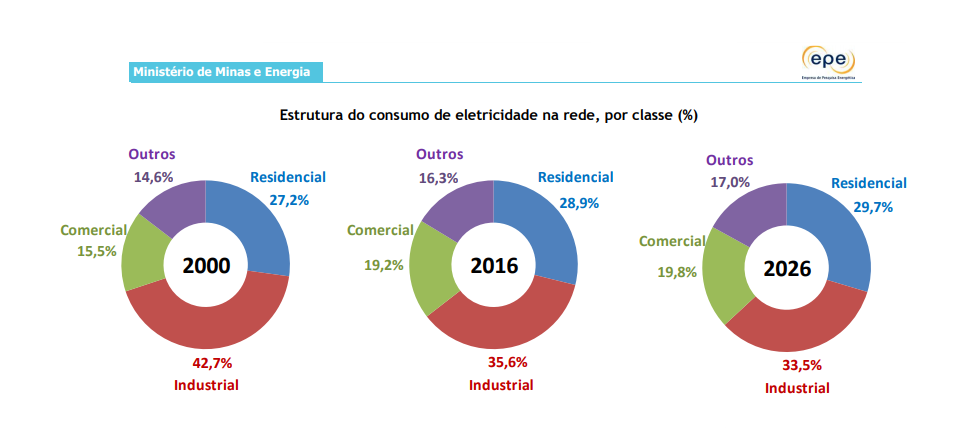
\includegraphics [scale=0.2]{./Figures/t02}
  	\end{center}
  \end{figure}
  \begin{figure}[h]
  	\begin{center}
      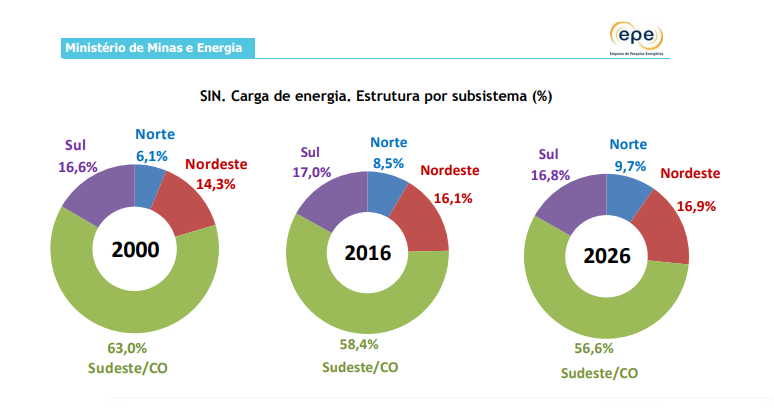
\includegraphics [scale=0.2]{./Figures/t03}
  	\end{center}
  \end{figure}
\end{frame}

\begin{frame}
  \begin{block}{}
   \begin{itemize}
      \item Compensação de Energia Elétrica com as Condições Gerais de
        Fornecimento (Resolução Normativa nº 414/2010).
   \end{itemize}
  \end{block}
  \begin{figure}[h]
  	\begin{center}
      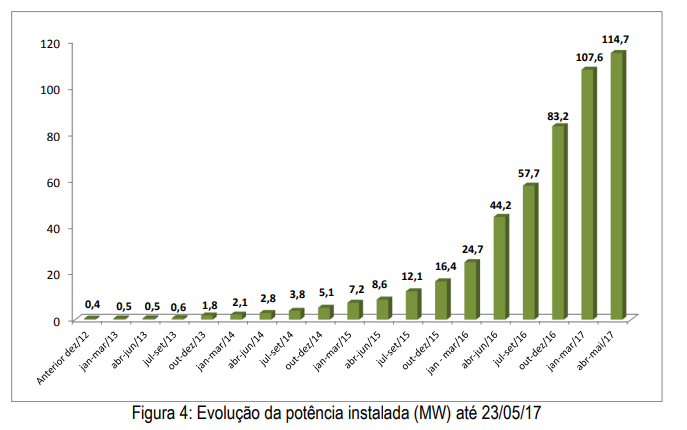
\includegraphics [scale=0.3]{./Figures/t04}
  	\end{center}
  \end{figure}
\end{frame}

\begin{frame}
  \begin{block}{}
   \begin{itemize}
        \item Aumento da quantidades de fontes na rede.
        \item Projeção de crescimento para os próximos anos.
        \item Maior disponibilidade de energia.
   \end{itemize}
  \end{block}
	\begin{figure}[!htb]
		\centering
		\subfloat[]{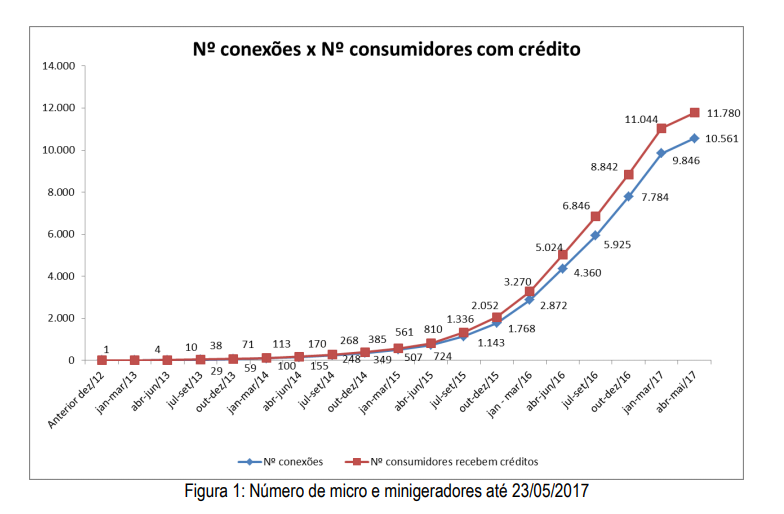
\includegraphics[height=3.4cm]{./Figures/t05}}
		\quad %espaco separador
		\subfloat[]{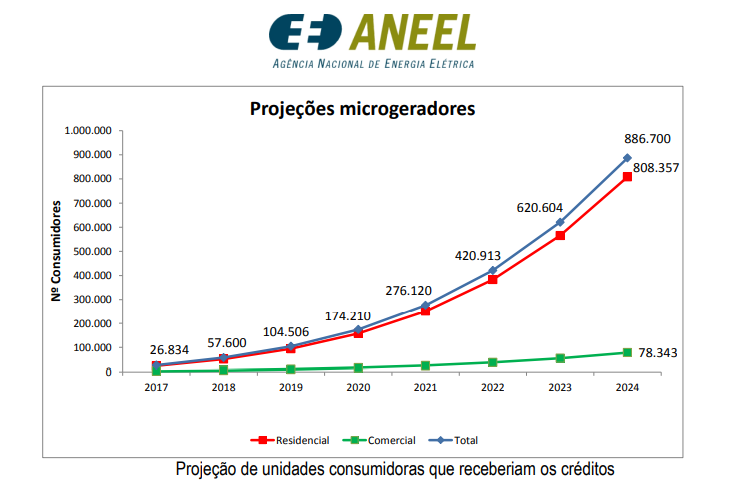
\includegraphics[height=3.4cm]{./Figures/t06}}
	\end{figure}
\end{frame}

\begin{frame}
  \begin{block}{}
   \begin{itemize}
     \item Fonte solar responde por 70\% e a eólica por 9\%.
   \end{itemize}
  \end{block}
	\begin{figure}[!htb]
		\centering
		\subfloat[]{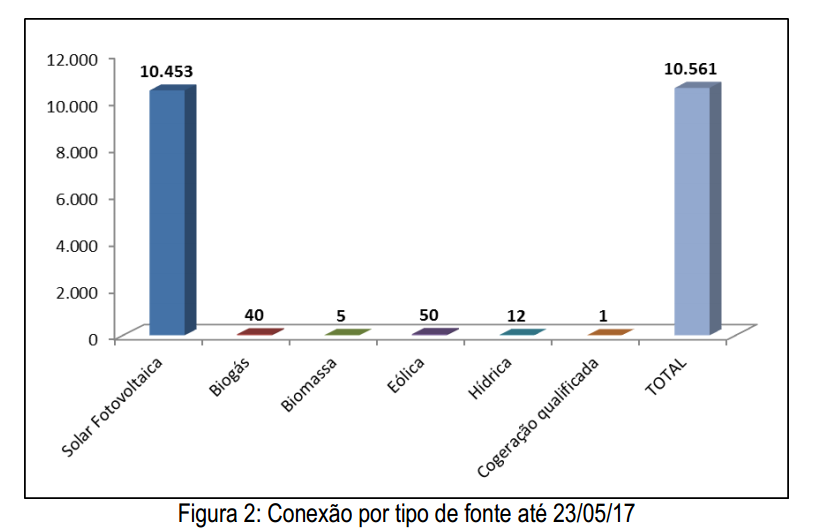
\includegraphics[height=3.4cm]{./Figures/t07}}
		\quad %espaco separador
		\subfloat[]{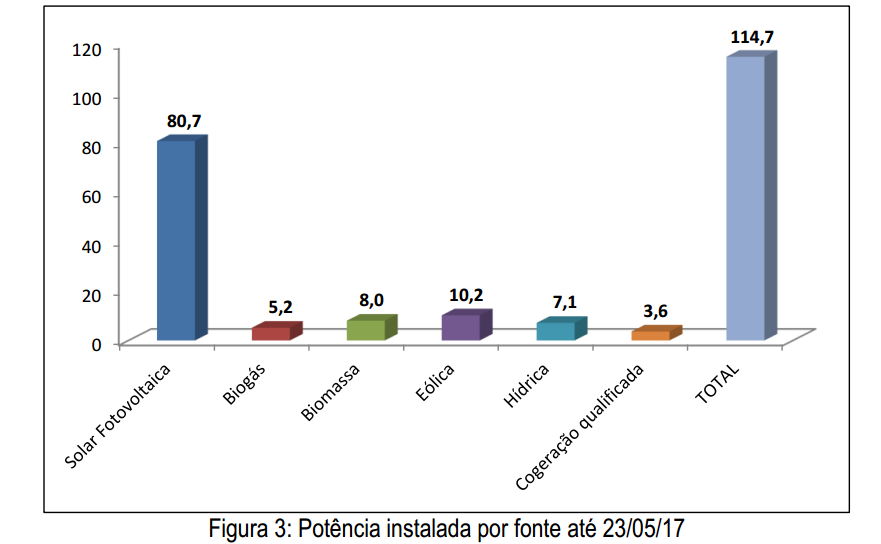
\includegraphics[height=3.4cm]{./Figures/t08}}
	\end{figure}
\end{frame}

\begin{frame}
  \begin{block}{}
   \begin{itemize}
     \item Deslocamento de carga par a horários com menor demanda e máxima
       geração local.
     \item Nota Técnica n 0056/2017-SRD/ANEEL
   \end{itemize}
  \end{block}
  \begin{figure}[h]
  	\begin{center}
      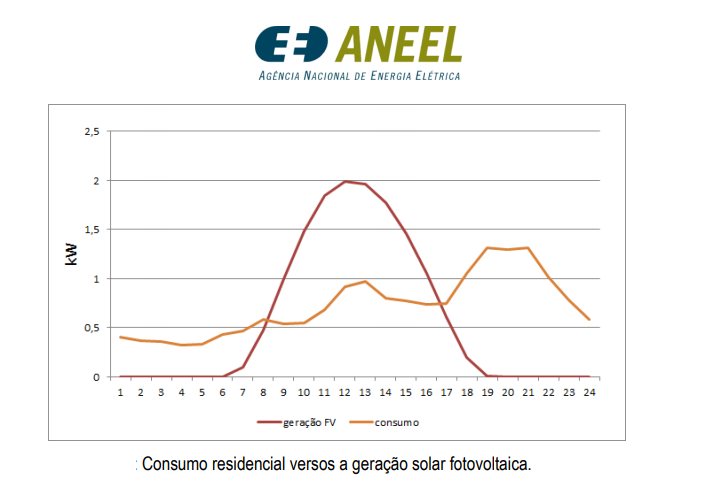
\includegraphics [scale=0.3]{./Figures/t09}
  	\end{center}
  \end{figure}
\end{frame}

\begin{frame}
  \begin{block}{Fundo do Clima BNDES}
   \begin{itemize}
     \item Financiamento à aquisição e à produção de máquinas e equipamentos
      com maiores índices de eficiência energética.
   \end{itemize}
  \end{block}
  \begin{figure}[h]
  	\begin{center}
      
\includegraphics [scale=0.3]{./Figures/t10}
  	\end{center}
  \end{figure}
\end{frame}

\begin{frame}
  \begin{block}{Conclusões}
   \begin{itemize}
     \item Os resultados diretos/indiretos sobre a realocação ótima de cargas
       em relação a demanda.
       \begin{itemize}
         \item Redução de custos gerais com energia.
         \item Reajuste tarifário com menor impacto \%.
         \item Melhores níveis de tensão.
         \item Aumento do número de fonte renováveis grade de geração.
         \item Redução de custos para companhias de energia elétrica com
           expansão de redes.
         \item Melhor eficiência sobre o carregamento de transformadores.
       \end{itemize}
   \end{itemize}
  \end{block}
\end{frame}

%\begin{frame}
%  \begin{figure}[h]
%  	\begin{center}
%      \includegraphics [scale=0.3]{./Figures/Device-Estimates}
%     % \caption {Estimativa de dispositivos conectados à Internet.}
%  		%\label{fig:arq-imuno}
%  	\end{center}
%  \end{figure}
%\end{frame}

%\begin{frame}{Redes de Acesso}
%	\begin{figure}[!htb]
%		\centering
%		\subfloat[DSL]{
%			\includegraphics[height=3.5cm]{./Figures/DSLaccess}
%			\label{figdroopy}}
%		\quad %espaco separador
%		\subfloat[Cable]{
%			\includegraphics[height=3.5cm]{./Figures/CableAccess}
%			\label{figsnoop}}
%		%\caption{Subfiguras}
%		%\label{fig01}
%	\end{figure}
%\end{frame}

%\begin{frame}[fragile]
%\scriptsize
%\begin{verbatim}
%\end{verbatim}
%\end{frame}

%\begin{frame}{\textit{Socket Programming with TCP}}
%\scriptsize
%\lstinputlisting[language=Python, caption={TCP Server.}]{./code/upperServer/TCPserver.py}
%\end{frame}

